\documentclass{standalone}
\usepackage{tikz}
\begin{document}
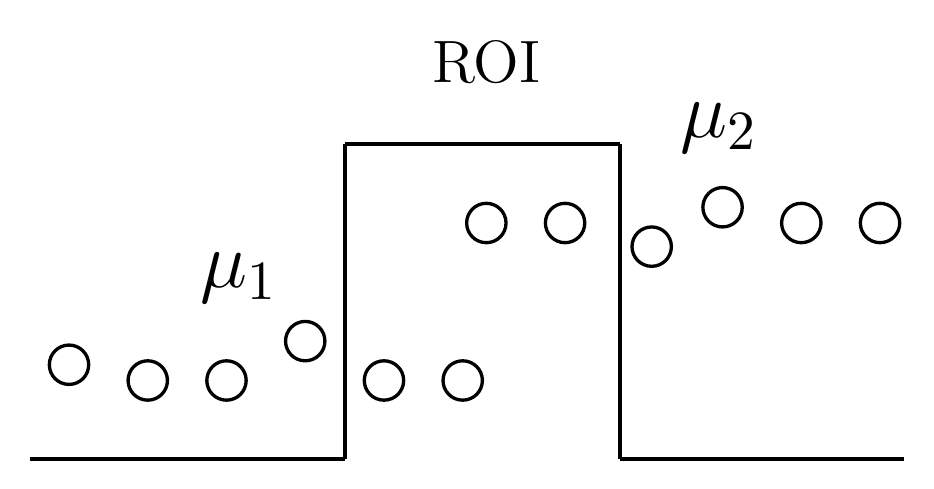
\begin{tikzpicture}[scale=1.0, xscale=1]
\def\rad{0.25}
\def\step{3}
%    \draw [<->] (0, 5) node [left] {$y$} -- (0,0) -- (15, 0) node [below right] at (15.5,-0.3) {$t$};
%\draw [->] (0,-0.5) -- (9,-0.5);
%\draw [->] (-1-2, -0.7) -- (-1-2,5);% node[left] {\Large Y};
%\draw [->] (-1.2-2, -0.5) -- (8.5, -0.5);% node[below] {\Large T};

\node[left, scale=2] at (0.9, 2.3) {\Large $\mu_1$};
\node[left, scale=2] at (7, 4.2) {\Large $\mu_2$};

\draw[fill=white, very thick] (-2, 1.2) circle (\rad);
\draw[fill=white, very thick] (-1, 1) circle (\rad);
\draw[fill=white, very thick] (0, 1) circle (\rad);
\draw[fill=white, very thick] (1, 1.5) circle (\rad);
\draw[fill=white, very thick] (2, 1) circle (\rad);
\draw[fill=white, very thick] (3, 1) circle (\rad);
\draw[fill=white, very thick] (3.3, \step) circle (\rad);
\draw[fill=white, very thick] (4.3, \step) circle (\rad);
\draw[fill=white, very thick] (5.4, \step-0.3) circle (\rad);
\draw[fill=white, very thick] (6.3, \step+0.2) circle (\rad);
\draw[fill=white, very thick] (7.3, \step) circle (\rad);
\draw[fill=white, very thick] (8.3, \step) circle (\rad);
%\draw[black, dashed] (4.5,0) -- (4.5, 4.5);

\draw[black, line width = 0.5mm] (-2.5, 0) -- (1.5, 0);
\draw[black, line width = 0.5mm] (1.5, 0) -- (1.5, 4);
\draw[black, line width = 0.5mm] (1.5, 4) -- (5.0, 4);
\draw[black, line width = 0.5mm] (5.0, 4) -- (5.0, 0);
\draw[black, line width = 0.5mm] (5.0, 0) -- (8.6,0);

%\draw[<->] (2.5, 4.6) -- (4.0, 4.6);
\node[above, scale=1.5] at (3.3, 4.6) {\Large ROI};

%\node[above] at (-2, 3.6) {\Large A};

\end{tikzpicture}
\end{document}
